\chapter{Introduction}
\label{sec:theory}

\section{The Standard Model of particle physics}

The Standard Model (SM) is a quantum field theory governing the kinematics and interactions of a set of fermion fields, respecting Lorentz and local gauge symmetries.
The gauge symmetries correspond to the SM gauge group:
\begin{equation}
 G = \SU(3) \times \SU(2) \times \U(1)
\end{equation}
This group can be decomposed into two subgroups: the \emph{strong} interaction governed by $\SU(3)$~\cite{qcd1,qcd2} and the \emph{electroweak} interaction governed by $\SU(2)\times\U(1)$~\cite{weak1,weak2,weak3}.
The action of $G$ on a fermion depends on the representation of the Lie group in which the fermion resides and the coupling strength.
For the special unitary groups, we denote the representation as $\mathbf{N}$ (fundamental), $\bar{\mathbf{N}}$ (anti-fundamental), or $\mathbf{1}$ (trivial).
The special unitary gauges have the same interaction strength for all fermions in non-trivial representations, known as \emph{universality}.
All fermions are in a one-dimensional representation of $\U(1)$, but the weak hypercharge $Y$ distinguishes their transformation under the gauge group $f\mapsto f + i Y g' f$, where $g'$ is the coupling strength of $\U(1)$.

Table~\ref{tab:theory:fermions} gives a summary of the \emph{first generation} SM fermion fields and the representation of $G$ which acts on them.
The SM provides a total of 3 generations of fermions, each of them a copy of the first generation in terms of the field content and gauge group action.

\begin{table}[]
\begin{center}
    \caption{First generation SM fermions and the action of the SM local gauge symmetry group $G$.
             The subscripts $L$ and $R$ refer to left- and right-handed chirality fields.
             Not shown are the charge conjugated fields $f^C \equiv Cf$, which sit in conjugated representations.}
    \label{tab:theory:fermions}
    \begin{tabular}{l|c|c|c|c}
                Name & Symbol       & $Y$ & $\SU(2)$ rep. & $\SU(3)$ rep. \\
                \hline \hline
  Left-handed lepton & $\ell_L$     & $-\nicefrac{1}{2}$  & $\mathbf{2}$  & $\mathbf{1}$ \\  
 Right-handed charged lepton & $e_R^-$   & $-1$  & $\mathbf{1}$  & $\mathbf{1}$ \\  
 Right-handed neutrino & $\nu_R$   & $0$  & $\mathbf{1}$  & $\mathbf{1}$ \\  \hline
  Left-handed quark  & $q  _L$     & $\nicefrac{1}{6}$  & $\mathbf{2}$  & $\mathbf{3}$ \\  
 Right-handed up quark  & $u  _R$     & $\nicefrac{2}{3}$  & $\mathbf{1}$  & $\mathbf{3}$ \\ 
 Right-handed down quark  & $d  _R$     & $-\nicefrac{1}{3}$  & $\mathbf{1}$  & $\mathbf{3}$ \\  
    \end{tabular}
\end{center}
\end{table}

The lepton doublets contain the left-handed charged leptons and neutral neutrinos:
\begin{equation}
    \ell_{iL} = 
    \left(\begin{matrix} \nu_e \\ e_L^- \end{matrix}\right),
    \left(\begin{matrix} \nu_\mu \\ \mu_L^- \end{matrix}\right),
    \left(\begin{matrix} \nu_\tau \\ \tau_L^- \end{matrix}\right)
\end{equation}
where $i$ indexes the generation.
The right handed lepton singlets contain the right-handed projections of the same fermions.

The quark (electroweak) doublets contain the left-handed up- and down-type quarks:
\begin{equation}
    q_{iL} = 
    \left(\begin{matrix} u_L \\ d'_L \end{matrix}\right),
    \left(\begin{matrix} c_L \\ s'_L \end{matrix}\right),
    \left(\begin{matrix} t_L \\ b'_L \end{matrix}\right)
\end{equation}
where $d'$, $s'$, and $b'$ represent linear combinations of the mass eigenstates $d$, $s$, and $b$ (discussed further in Section~\ref{sec:theory:ew}).
All quarks also sit in a strong triplet; we have suppressed its charge above, as the strong representation is orthogonal to the electroweak representation.
Where necessary, it will be specified with a superscript, i.e. $u^{c}$.

\subsection{Quantum chromodynamics}
The dynamics of quarks under the $\SU(3)$ gauge group are commonly referred to as the strong interaction or quantum chromodynamics (QCD).
The QCD Lagrangian is:
\begin{equation}
    \mathcal{L}_\mathrm{QCD} = 
        i \bar q^{a}_f \slashed D^{ab} q^{b}_f  
        + m_f \bar{q}^{a}_f q^{a}_f
        - \frac{1}{4} G^{a}_{\mu\nu} G^{a,\mu\nu}
    \label{eq:theory:lqcd}
\end{equation}
where repeated indices are contracted; $q_f=u,d,c,s,b,t$ are the spinors for each quark flavor $f$; $a,b=r,g,b$ index the basis elements of the triplet representation, called \emph{colors}; $m_q$ is the mass of quark flavor $q$.
$D_\mu$ is the QCD covariant derivative:
\begin{equation}
    D_\mu^{ab} = \delta^{ab} \partial_\mu - i g_s \sum_c t^{ab}_c G_{c,\mu}
\end{equation}
where $g_s$ is the strong coupling strength; $t_c$ are the 8 generators of the triplet representation of $\SU(3)$; $G_c$ are the corresponding 8 gauge boson (gluon) fields. 
$G^a_{\mu\nu}$ are the gluon field strength tensors:
\begin{equation}
    G^a_{\mu\nu} = \partial_\mu G_\nu^a - \partial_\nu G_\mu^a - g_s f^{abc} G_\mu^b G_\nu^c
\end{equation}
where $f^{abc}$ are the structure constants of $\SU(3)$, with $a,b,c=r,g,b$.

An additional term can be added to Equation~\ref{eq:theory:lqcd} without violating any guage or Lorentz symmetry or renormalizability.
This term would violate CP conservation and produce a non-zero electric dipole moment (EDM) for the neutron.
No evidence for such a term has yet been found, although it has not been excluded~\cite{nedm1}
We therefore do not consider it as part of the SM QCD Lagrangian. 

\subsubsection{Renormalization and running of couplings}

Physical quantities in a QFT such as couplings and masses acquire a scale-dependence from higher-order corrections to vertices and propagators. 
In many cases, the quantum corrections to the bare parameter contain ultraviolet divergent terms.
These infinities are absorbed into the Lagrangian by means of adding \emph{counterterms}. 
The systematic process of absorbing these infinities and ensuring scale-independence is known as renormalization.
A Lagrangian is called \emph{renormalizable} if only a finite number of counterterms are needed to ensure that all observables (i.e. amplitudes) are finite. 
The SM is a renormalizable theory.

In this discussion, we will focus on the renormalization of the coupling $\alpha_S \equiv \nicefrac{g_s^2}{4\pi}$, but the argument applies broadly to all SM quantities.
There are two related consequences of quantum corrections.
Firstly, $\alpha_S$ acquires a non-trivial dependence on the probed energy scale $\mu_R^2 = -q^2$, where $q^\mu$ is the momentum transferred by the gluon.
Secondly, the \emph{bare} $\alpha_S$ as written in the Lagrangian is not the same as the $\alpha_S(\mu_R^2)$ measured in the laboratory.
We will refer to the bare coupling as $\alpha_{S0}$. 
Note that it does not have a $\mu_R^2$-dependence.
To enforce this, we look for solutions to the differential equation
\begin{equation}
    \mu_R^2 \frac{\di \alpha_{S0}}{\di\mu_R^2} = 0
\end{equation}
Writing $\alpha_{S0}$ in terms of $\alpha_S$, which has a $\mu_R^2$-dependence, and rearranging the terms gives the \emph{$\beta$ function} for $\alpha_S$:
\begin{equation}
    \beta(\alpha_S) \equiv \mu_R^2 \frac{\di \alpha_S}{\di\mu_R^2} = -\left(\beta_0 \alpha_S^2 + \beta_1 \alpha_S^3 + \mathcal{O}(\alpha_S^4)\right)
\end{equation}
The $\beta$ coefficients are:
\begin{align}
    \beta_0 = \frac{33 - 2n_{f}}{3},~ 
    \beta_1 = \frac{153-19n_f}{24\pi^2} ,\dots
\end{align}
where $n_f$ is the number of quark flavors with masses below $\mu_R$~\cite{pdg,qcd1,qcd2,qcd3}.
To one-loop order, the solution to this differential equation is:
\begin{equation}
    \alpha_S(\mu_R) = \frac{2\pi}{\beta_0 \ln \frac{\mu_R}{\Lambda_\mathrm{QCD}}}
\end{equation}
where $\Lambda_\mathrm{QCD}$ is set by enforcing a measured boundary condition, e.g. $\alpha_S(m_Z^2) = 0.1181 \pm 0.0011$~\cite{pdg}.
Using $n_f=5$ at $\mu_R = m_Z$ and the $\overline{\text{MS}}$ renormalization scheme~\cite{msbar} gives $\Lambda_\mathrm{QCD} = 218$ MeV.
$\beta_0>0$ implies $\alpha_S$ falls as a function of energy, as illustrated in Figure~\ref{fig:theory:alphas}.

This running is the opposite of theories like quantum electrodynamics, in which $\beta_0<0$.
It results in an asymptotically free theory as $\mu_R\rightarrow \infty$.
Below $\Lambda_\mathrm{QCD}$, the coupling constant is larger than order unity.
In the regime where $\alpha_S < 1$, perturbation theory can be applied to calculate observables with $\alpha_S$ as the expansion parameter.
This is referred to as perturbative QCD (pQCD).
The long-range behavior of QCD also means that quarks and gluons, which have a color charge, cannot be observed below a temperature $\sim 10^{12}$ K~\cite{hagedorn}.
Instead, a spectrum of composite color singlet states, known as \emph{hadrons}, are observed~\cite{quarkmodel}.

\begin{figure}[]
\begin{center}
    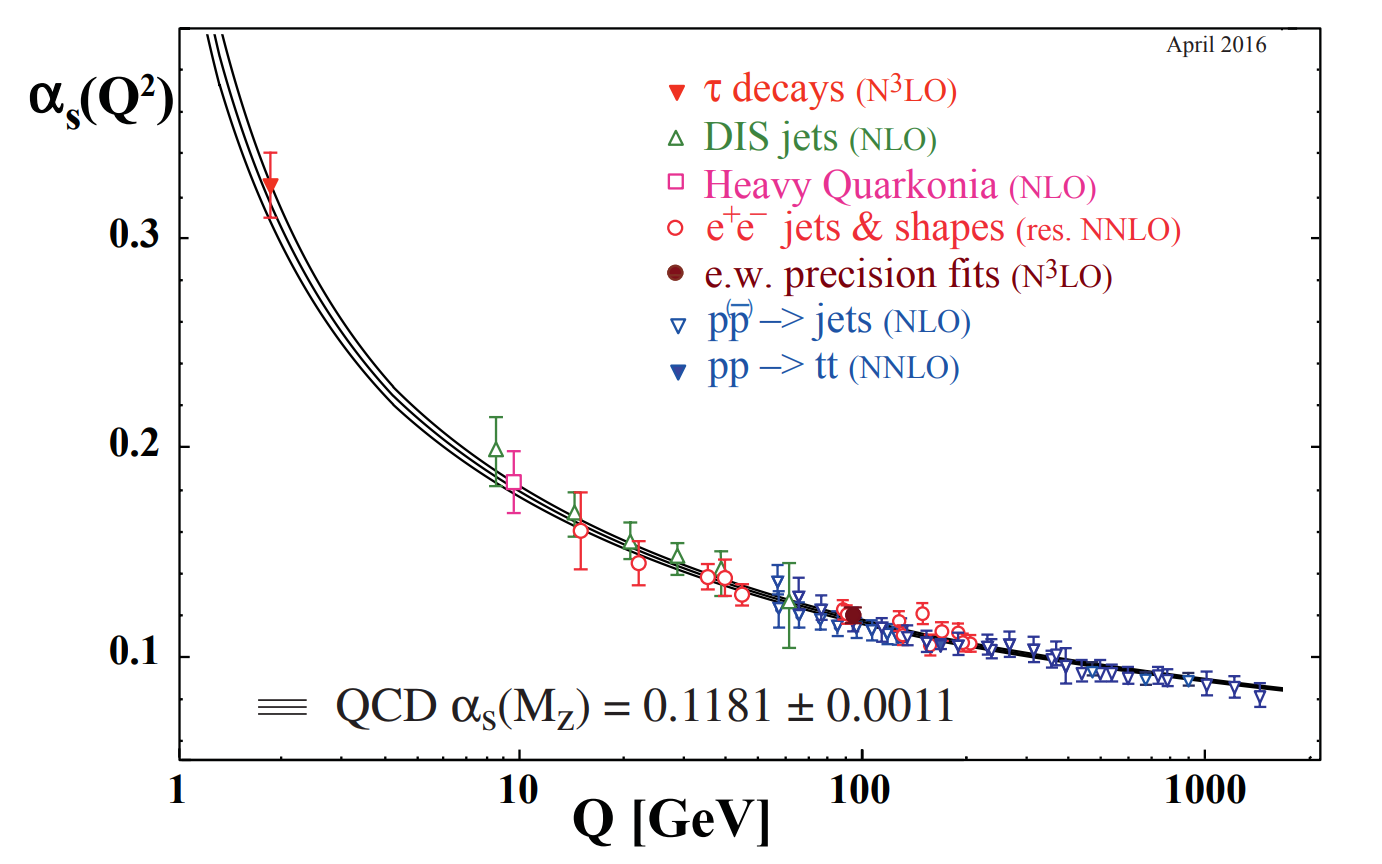
\includegraphics[width=0.6\textwidth]{figures/theory/alphas.png}
    \caption{Running of the QCD coupling strength $\alpha_S$ as a function of length scale.
             Reprinted from Reference~\cite{pdg}.}
    \label{fig:theory:alphas}.
\end{center}
\end{figure}

\subsection{Electroweak interactions}
\label{sec:theory:ew}
The electroweak (EW) sector of the SM refers to the $\SU(2)\times\U(1)$ symmetry group.
While all fermion fields in Table~\ref{tab:theory:fermions} transform under $\U(1)$, only left-handed fermions have non-trivial transformations under $\SU(2)$.
Ignoring mass terms and the Higgs sector, the EW Lagrangian is:
\begin{align}
\mathcal{L}_\mathrm{EW} =~
        & i\bar\ell_{iL} \left(\slashed\partial-ig \slashed W^a \tau^a - ig'Y_{\ell_L} \slashed B\right)\ell_{iL} 
      + i\bar q_{iL}^{c} \left(\slashed\partial-ig \slashed W^a \tau^a - ig'Y_{q_L} \slashed B\right)q_{iL}^{c} \nonumber \\
      & + i\bar e_{iR} \left(\slashed\partial-ig'Y_{ e_R}\slashed B\right) e_{iR} 
       + i\bar u_{iR^{c}} \left(\slashed\partial-ig'Y_{u_R}\slashed B\right) u_{iR}^{c} 
       + i\bar d_{iR}^{c} \left(\slashed\partial-ig'Y_{d_R}\slashed B\right) d_{iR}^{c} \nonumber \\ 
      & - \frac{1}{4} W_{\mu\nu}^a W^{a,\mu\nu} - \frac{1}{4} B_{\mu\nu} B^{\mu\nu}  
      \label{eq:theory:lew}
\end{align}
where repeated indices are contracted; the subscript $i$ indexes generations; $g$ and $g'$ are respectively the coupling strengths for $\SU(2)$ and $\U(1)$; $Y$ is the weak hypercharge; $W_\mu^a$ are the three gauge fields corresponding to the generators $\tau^a = \nicefrac{\sigma^a}{2}$ of $\SU(3)$; $B_\mu$ is the gauge field for $\U(1)$; and $W_{\mu\nu}^a$ and $B_{\mu\nu}$ are the field strength tensors for the respective gauge fields.
The covariant derivative can be written as:
\begin{equation}
    D_\mu = \partial_\mu - ig\delta_L W^a_\mu \tau^a - ig' YB_\mu
\end{equation}
where $Y$ is the particle's hypercharge and $\delta_L$ is 1 if the field is in the $\mathbf{2}$ representation of $\SU(2)$ (e.g. left-handed fermions) and 0 otherwise. 

\subsubsection{EW symmetry breaking}
Unlike Equation~\ref{eq:theory:lqcd}, we cannot introduce a quadratic mass term for fermions in Equation~\ref{eq:theory:lew} because $\bar\psi \psi = \psi^\dag_R\psi_L + \psi^\dag_L\psi_R$ is not invariant under $\SU(2)$ rotations.
Spontaneous electroweak symmetry breaking remedies this, as well as provides masses for the gauge fields~\cite{ewsb1,ewsb2,ewsb3,ewsb4,ewsb5,ewsb6}.
A complex scalar doublet $\phi$ (called the complex Higgs field) with $Y_\phi=\nicefrac{1}{2},~\delta_L=1$ is added to the Lagrangian:
\begin{equation}
    \mathcal{L}_\mathrm{EW} \mapsto \mathcal{L}_\mathrm{EW}
            + |D_\mu \phi|^2 + \mu^2|\phi|^2 - \lambda |\phi|^4
    \label{eq:theory:lhiggs}
\end{equation}
We can write the complex doublet as 4 real fields:
\begin{equation}
    \phi = \frac{1}{\sqrt{2}} \left(\begin{matrix} \phi_1 + i\phi_2 \\ \phi_3 + i \phi_4 \end{matrix} \right)
\end{equation}
The two self-interaction terms create a Higgs potential with a degenerate global minimum at \emph{vacuum expectation value} $v \equiv \langle |\phi| \rangle = \sqrt{\nicefrac{\mu^2}{\lambda}}$.
Through gauge rotations, we can fix $\langle\phi_{1,2,4}\rangle = 0$ and, at low energies, expand $\phi_3 = v + H$, where $H$ is the real Higgs field. 
This is the spontaneous breaking of a symmetry.

By the Nambu-Goldstone theorem~\cite{nambu,goldstone}, these three lost degrees of freedom give rise to three massless bosons. 
The $|D_\mu \phi|$ term couples the complex Higgs field to the gauge bosons:
\begin{align}
    |D_\mu \phi|^2_{\phi = \langle\phi\rangle} &= 
        \frac{v^2}{8} \left[(gW_\mu^1)^2 + (gW^2_\mu)^2 + (g'B_\mu - gW_\mu^3)^2\right] 
\end{align}
The diagonalization of this mass term gives 3 massive weak bosons (consuming the 3 massless Nambu-Goldstone bosons) and one massless photon:
\begin{align}
    W^\pm_\mu &\equiv \frac{W_\mu^1 \mp iW_\mu^2}{\sqrt{2}} \nonumber \\ 
    Z_\mu &\equiv \cos\theta_w W_\mu^3 - \sin\theta_w B_\mu \nonumber \\ 
    A_\mu &\equiv \sin\theta_w W_\mu^3 + \cos\theta_w B_\mu
\end{align}
where $\tan\theta_w = g'/g$.
The corresponding mass eigenvalues are:
\begin{equation}
    m_W = \frac{gv}{2}, \quad m_Z = \frac{v\sqrt{g^2+g'^2}}{2}, \quad m_A = 0
\end{equation}

The remaining $H$ field, which has not been consumed, gives rise to the Higgs boson discovered by CMS and ATLAS~\cite{higgsdisc} in 2012.
It has mass $m_H = \sqrt2\mu$.
By expanding $\phi$ around $\langle \phi \rangle$ in Equation~\ref{eq:theory:lhiggs}, we find couplings to the massive gauge bosons:
\begin{gather}
    \frac{m_Z^2}{v} hZ_\mu Z^\mu, \quad \frac{2m_W^2}{v}hW^{+\mu} W^{-}_\mu, \nonumber \\
    \frac{m_Z^2}{2v} h^2 Z_\mu Z^\mu, \quad \frac{m_W^2}{v} h^2 W^{+\mu} W^-_\mu 
\end{gather}
The breaking of the $\SU(2)\times \U(1)$ symmetry leaves behind the local $\U(1)$ symmetry of electromagnetism (EM), with gauge boson $A_\mu$.
Fermions have EM charge $eQ = e(T_3+Y)$, where $e=g'\cos\theta_w$ and $T_3$ is the third isospin component. 
The $W^\pm$ bosons receive charge $\pm e$.
After symmetry breaking, the actions of the broken gauge groups on fermions are governed by the following Lagrangian terms:
\begin{align}
    \La_\mathrm{EWSB} \supset 
            \sum_f &\left[\bar f\left(i\slashed\partial-eQ_f\slashed A\right) f 
            - \frac{g}{2\sqrt{2}} \bar f_L \left(T^+\slashed W^+ + T^- \slashed W^-\right) f_L\right. \nonumber \\
            &\left.~- \frac{g}{2\cos\theta_w} \bar f\left(g_{Vf} - g_{Af} \right)\slashed Z f \right]
\end{align}
where $f$ are all fermion fields; $f_L = \frac{1}{2}(1-\gamma^5)f$; $g_{V} = T_3- 2Q\sin^2\theta_w$; and $g_{A} = T_3$.

\subsubsection{Fermion masses}
The last piece of the EW Lagrangian is the addition of the fermion masses through Yukawa couplings with the Higgs doublet. 
First, let us add the terms for quark couplings:
\begin{equation}
   \La_\mathrm{EW} \mapsto \La_\mathrm{EW} - y_{ij}^d \bar q_{iL} \phi d_{jR} - y_{ij}^u \bar q_{iL}i\sigma_2 \phi^* u_{uR}i + \hc
\end{equation}
where $\hc$ refers to the Hermetian conjugate of preceding terms; and $y_{ij}^{u,d}$ are the Yukawa matrices for up- and down-type quarks.
Breaking the symmetry and collecting terms proportional to $v$:
\begin{equation}
    -\frac{v}{\sqrt{2}}\left(y_{ij}^d \bar d_{iL}' d_{jR} + y_{ij}^u \bar u_{iL} u_{jR}\right) 
\end{equation}
The mass eigenstates are found by diagonalizing these terms, which are written in terms of the weak eigenstates.
Let us denote the unitary transformations from the mass basis to the weak basis as $U_u$ and $U_d$. 
If we try to write the rest of $\La_\mathrm{EWSB}$ in terms of mass eigenstates, we see that terms of the following form all have trivial transformations:
\begin{gather} 
\bar d' \gamma^\mu d' \mapsto \bar d U_d^\dag \gamma^\mu U_d d = \bar d \gamma^\mu d
\end{gather}
The only non-trivial transformation is in the charged weak interaction:
\begin{align} 
\bar u_L \slashed W^+ d'_L + \bar d'_L W^- u_L &\mapsto 
    \bar u_L \slashed W^+ U_u^\dag U_d d_L + \bar d_L W^- U_d^\dag U_u u_L \nonumber \\
    &\equiv \bar u_L \slashed W^+ V_\mathrm{CKM} d_L + \bar d_L W^- V^\dag_\mathrm{CKM} u_L
\end{align}
where $V_\mathrm{CKM}$ is the Cabibbo-Kobayshi-Maskawa matrix~\cite{ckm1,ckm2}.
It is nearly-diagonal, but with non-zero mixing between the generations. 
The CKM matrix also contains a charge parity (CP) violating phase.
When referring to down-type quarks, we typically refer to the mass eigenstate $d$ as opposed to $d'$.

A similar analysis can be carried out for the lepton sector:
\begin{equation}
   \La_\mathrm{EW} \mapsto \La_\mathrm{EW} - y_{ij}^e \bar \ell_{iL} \phi e_{jR} - y_{ij}^\nu \bar \ell_{iL}i\sigma_2 \phi^* \nu_{uR}i + \hc
\end{equation}
The mixing matrix for leptons is the Pontecorvo-Maki-Nakagawa-Sakata matrix $U_\mathrm{PMNS}$ \cite{pmns}, which relates the weak eigenstates $\nu_e, \nu_\mu,\nu_\tau$ with the mass eigenstates $\nu_1,\nu_2,\nu_3$.
The values of the neutrino masses are known to be non-zero from the observation of neutrino oscillations~\cite{nuosc}.

After EWSB, each fermion mass eigenstate has a mass term and coupling to the Higgs field:
\begin{equation}
    \La_\mathrm{EWSB} \supset \sum_f -\frac{y_f v}{\sqrt{2}} \left( \bar ff + \bar fH f\right)
\end{equation}
where we identify the mass as $m_f = y_f v/\sqrt{2}$. 
Table~\ref{tab:theory:ewsb} summarizes all SM fermions and some of their properties after EWSB.

\begin{table}[]
\begin{center}
    \caption{Summary of the SM fields after electroweak symmery breaking.
             All masses are taken from the global fits compiled by the Particle Data Group~\cite{pdg}.}
    \label{tab:theory:ewsb}
    \begin{tabular}{l|c|c|c|c}
        Name & Symbol & Spin & Mass & $Q_e$  \\  \hline \hline
        gluon & $g^{ab}$ & 1 & 0 & 0 \\   
        photon & $\gamma $ & 1 & 0 & 0 \\   
        $Z$ boson & $Z$ & 1 & 91.2 GeV & 0 \\   
        $W$ boson & $W^{\pm}$ & 1 & 80.4 GeV & $\pm 1$ \\   \hline 
        Higgs boson & $H$ & 0 & 125 GeV & $0$ \\   \hline 
        up quark & $u$ & $\nicefrac{1}{2}$ & $2.2$ MeV & $\nicefrac{2}{3}$    \\   
        down quark & $d$  & $\nicefrac{1}{2}$ & $4.7$ MeV  & $-\nicefrac{1}{3}$  \\   
        charm quark & $c$  & $\nicefrac{1}{2}$ & $1.28$ GeV  & $\nicefrac{2}{3}$  \\   
        strange quark & $s$  & $\nicefrac{1}{2}$ & $95$ MeV  & $-\nicefrac{1}{3}$  \\   
        top quark & $t$  & $\nicefrac{1}{2}$ & $173$ GeV  & $\nicefrac{2}{3}$  \\  
        bottom quark & $b$  & $\nicefrac{1}{2}$ & $4.18$ GeV  & $-\nicefrac{1}{3}$  \\   \hline
        electron neutrino  & $\nu_e$  & $\nicefrac{1}{2}$ & $-$  & $0$  \\   
        electron  & $e$  & $\nicefrac{1}{2}$ & $511$ keV  & $-1$  \\   
        muon neutrino  & $\nu_\mu$  & $\nicefrac{1}{2}$ & $-$  & $0$  \\   
        muon  & $\mu$  & $\nicefrac{1}{2}$ & $105$ MeV  & $-1$  \\   
        tau neutrino  & $\nu_\tau$  & $\nicefrac{1}{2}$ & $-$  & $0$  \\ 
        tau  & $\tau$  & $\nicefrac{1}{2}$ & $178$ GeV  & $-1$  \\   
    \end{tabular}
\end{center}
\end{table}

\section{Dark matter}

The SM is able to predict the outcomes of many laboratory experiments, ranging from measurements of the electron magnetic moment~\cite{eedm} to the discovery and characterization of the Higgs boson~\cite{higgsdisc,higgsprop}.
Nonetheless, there are certain classes of phenomena it cannot explain:
\begin{itemize}
    \item There is not yet a complete formulation of \emph{quantum gravity} that incorporates general relativity~\cite{gr}.
    \item The observed \emph{matter/antimatter asymmetry} in the universe cannot be explained by the SM's CP violation and (predicted) baryon number of violation. 
          Additional CP- and $B$-violating interactions must exist.
    \item \emph{Neutrino masses} are not completely determined by the SM. 
            While a mass term can be written down as in Section~\ref{sec:theory:ew}, it does not exclude a Majorana mass term for right-handed neutrinos. 
            Nor does it explain the observed range of masses $m_\nu/m_t \lesssim 10^{-15}$. 
    \item An explanation of \emph{dark energy} accounting for $\sim 68\%$ of the universe's energy budget, suggested by measurements of the CMB, galaxy clusters, supernovae, and other measurements of the universe expansion rate~\cite{darkenergy}.
    \item An explanation of \emph{dark matter} accounting for $\sim 27\%$ of the universe's energy budget, suggested by measurements of galactic rotation curves, the CMB, and gravitational lensing~\cite{pdg,dm1,dm2,dm3}.
\end{itemize}
In this thesis, we describe tests of certain extensions of the SM which add candidate fields for dark matter (DM). 

\subsubsection{Astrophysical evidence}
All known evidence of DM arises from gravitational measurements.
One of the oldest observations is that of galactic rotational curves.
The rotational velocities of stars and hydrogen clouds are measured in galaxies, as a function of the distance from the center of the galaxy.
It is found that the velocity increases as a function of radius, eventually reaching a plateau that extends well past the bulk of the visible mass of the galaxy.
This implies the existence of a massive dark halo that encompasses the galaxy.
Indeed, the observed rotational curves $v(r)$ are well-described by a 3 component fit: the visible disk, a gas cloud, and a dark halo. 
Two galaxies are shown in Figure~\ref{fig:theory:dm_rot}, and it is clear that a non-zero DM component is needed to describe the data.

\begin{figure}[]
\begin{center}
    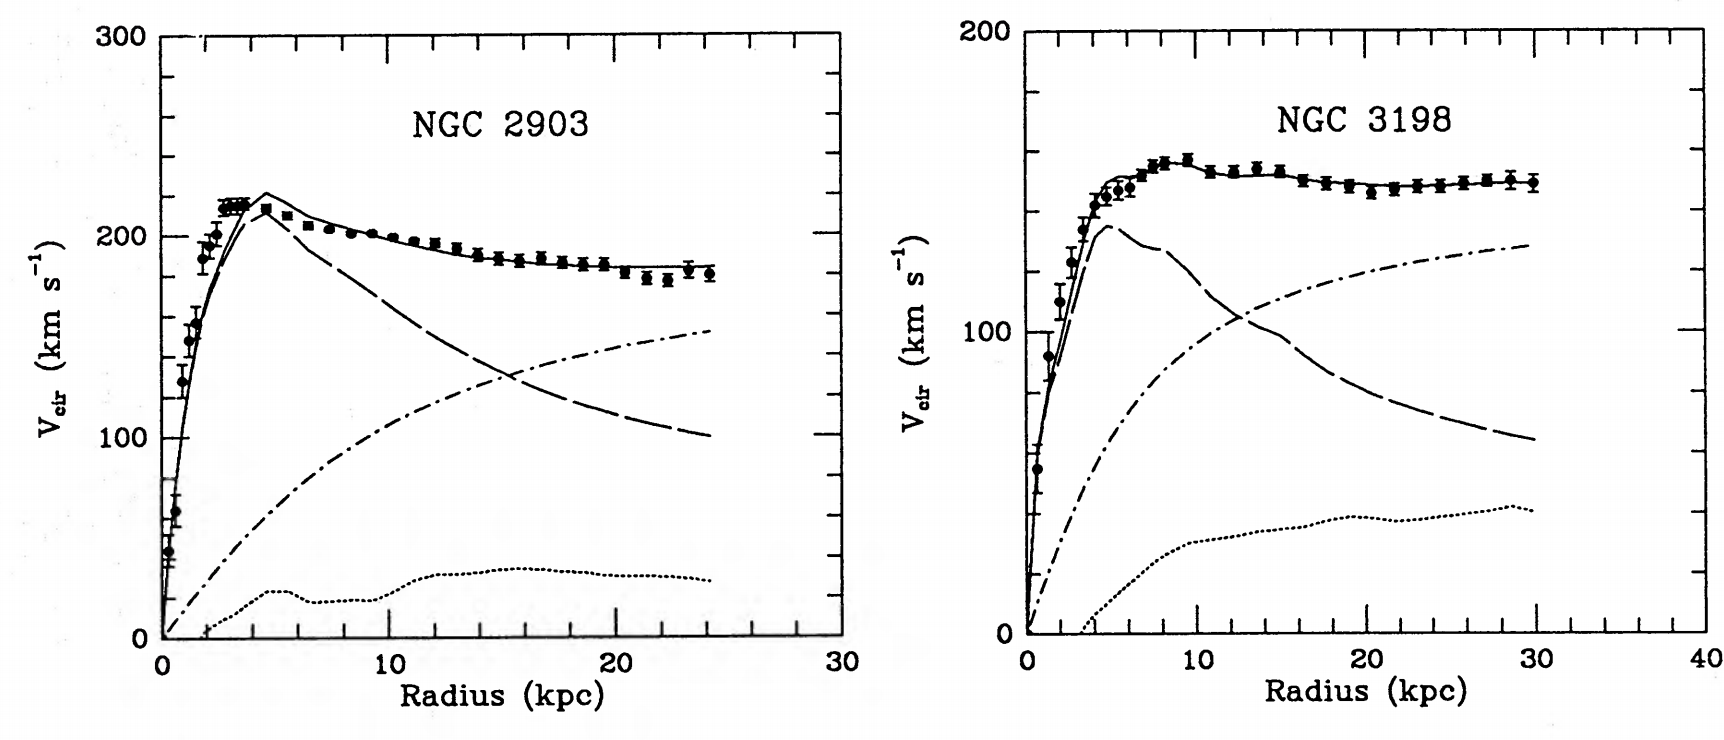
\includegraphics[width=0.7\textwidth]{figures/theory/dm_rot.png}
    \caption{Observed and fitted galactic rotational curves for two galaxies.
             The total fit (solid line) has three components: visible (dashed), gas clouds (dotted), and DM (dash-dotted). 
             Reprinted from Reference~\cite{dmrot}.}
    \label{fig:theory:dm_rot}
\end{center}
\end{figure}

An orthogonal piece of evidence comes from measuring anisotropies in the cosmic microwave background (CMB).
The CMB is the remnant of photons after they decoupled from matter in the early universe.
The temperature spectrum of the CMB is isotropic to one part in $10^5$, and the anisotropies are driven by matter anisotropies at the time of decoupling.
The power spectrum of the temperature anisotropies is modified when there are two matter populations (SM and DM) as opposed to one (just SM), especially when the two populations interact with each other via gravity, but one does not interact with photons (DM).
Figure~\ref{fig:theory:planck} shows the power spectrum measured by the Planck experiment~\cite{planck}, compared to the best-fit $\Lambda$ Cold Dark Matter ($\Lambda$CDM) model.

\begin{figure}[]
\begin{center}
    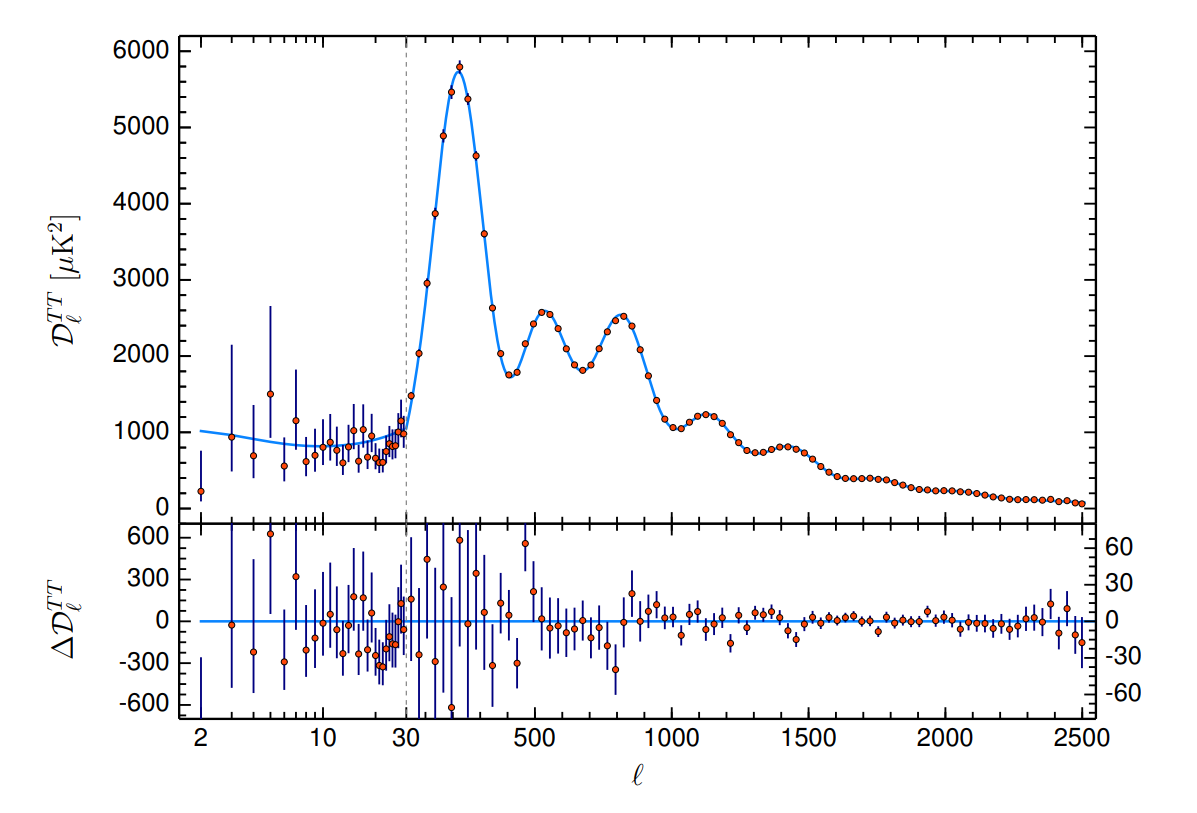
\includegraphics[width=0.7\textwidth]{figures/theory/planck.png}
    \caption{Temperature anisotropy power spectrum of the CMB, as measured by Planck.
             Reprinted from Reference~\cite{planck}.}
    \label{fig:theory:planck}
\end{center}
\end{figure}

This is hardly an exhaustive list of DM evidence.
Other observations include gravitational lensing, cluster collisions, and large-scale structure formation~\cite{dm1,dm2}.

\subsubsection{DM candidates}

The \emph{relic density} is the current density of a field that fell out of thermodynamic equilibrium with other fields as the universe expanded.
This occurs as the rate of expansion of the universe outpaces the mean particle velocity $v$ (correlated with the temperature $T$) and the cross sections for annihilation and production of the field.
This decoupling of the field is known as \emph{freeze-out}.
The relic density is defined:
\begin{equation}
    \Omega \cdot h^2 = \frac{\rho}{\rho_c} \cdot \frac{H_0}{100\text{ km/s/Mpc}}
\end{equation}
where $\rho$ is the energy density of the field, $\rho_c$ is the critical total energy density of flat spacetime, and $H_0=73$ km/s/Mpc is the Hubble constant.
If $\sigma_A$ is the annihilation cross section and the field is non-relativistic at freeze-out, then a very simplified approximation~\cite{dm1} is:
\begin{equation}
    \Omega h^2 = \frac{10^{-27}\mathrm{cm}^3\mathrm{s}^{-1}}{\langle \sigma_A v\rangle}
    \label{eq:theory:relic}
\end{equation}
Planck~\cite{planck} measures the relic densities of baryonic and dark matter to be:
\begin{equation}
    \Omega_b h^2 = 0.02237 \pm 0.0015, \quad \Omega_\mathrm{DM} h^2 = 0.1200 \pm 0.0012
\end{equation}

As a first candidate, suppose we introduce a fermion $\chi$ with mass $m_\chi\sim100$ GeV.
Further suppose that it has an interaction with the SM through a new current, and the cross section for the effective four-point interaction $\chi \bar\chi\rightarrow f\bar f$ (for some SM fermion $f$) is proportional to $g^4_\chi$, where $g_\chi \sim g \sim 0.6$.
The relic density for such a particle would be $\Omega_\chi h^2 \sim 0.1$, which is quite close to the needed density.
A \emph{Weakly-Interacting Massive Particle} (WIMP) such as $\chi$ therefore makes a good DM candidate.
This coincidence is known as the \emph{WIMP miracle}.
It should be noted that the definition of a WIMP is fairly loose.
All models considered in these results contain at least one particle falling under the umbrella of a WIMP, but the models themselves are quite diverse.

Many DM models other than WIMPs exist.
The obvious SM candidate for DM are neutrinos, as they are known to be non-interacting and massive.
However, constraints on the neutrino mass restrict $\Omega_\nu h^2 \leq 0.0062$~\cite{pdg}, which is far too small to entirely account for the observed phenomena. 
Sterile neutrinos (neutrinos that participate in oscillations but do not couple to the $Z$ boson) remain a viable DM candidate, above a mass of 10 keV.
Another DM hypothesis is a scalar \emph{axion} field, which also serves as a solution to the strong CP problem.
While axions can have couplings to photons, those interactions would be sufficiently weak for an axion to remain \emph{dark} in the sense of DM.
Many other DM candidates have been proposed as well (some of which fall under the generic WIMP umbrella), and this is not an exhaustive list.

\subsubsection{Non-collider WIMP searches}

Each class of DM models has dedicated experimental signatures, and therefore dedicated experiments to search for them.
The philosophy of collider DM searches is to produce DM in the laboratory and directly or indirectly detect it.
Here, we focus on searches sensitive to WIMPs, as these are most relevant for the results in this thesis.
The mass and coupling ranges of WIMPs allow the possibility for their production at a TeV-scale collider, such as the LHC.
In contrast, non-collider searches rely on DM that is present somewhere in the universe and look for its interaction with SM particles.

\emph{Indirect detection} experiments look for the annihilation process $\chi\bar\chi\rightarrow X$, where $X$ is one or more SM particles.
The Alpha Magnetic Spectrometer (AMS-02) searches for excess positrons in the cosmic ray flux, arising from $X=e^+e^-$ final states~\cite{ams}. 
Similarly, $\gamma$ ray data from the Fermi Large Area Telescope (Fermi-LAT) is used to look for final states which include high-energy photons~\cite{fermilat}.
As an example, the 95\% CL exclusion from Fermi-LAT is shown in Figure~\ref{fig:theory:fermilat}.
The exclusion is drawn as a function of $m_\chi$ and $\langle \sigma_A v\rangle$, as the Fermi-LAT analysis is directly dependent on the annihilation rate.
Also shown is an exclusion from a search conducted by the CMS experiment at the LHC, looking for the process $pp\rightarrow \chi+$jet and assuming a pseudoscalar mediator connecting the DM and SM sectors~\cite{monojet}.

\begin{figure}[]
\begin{center}
    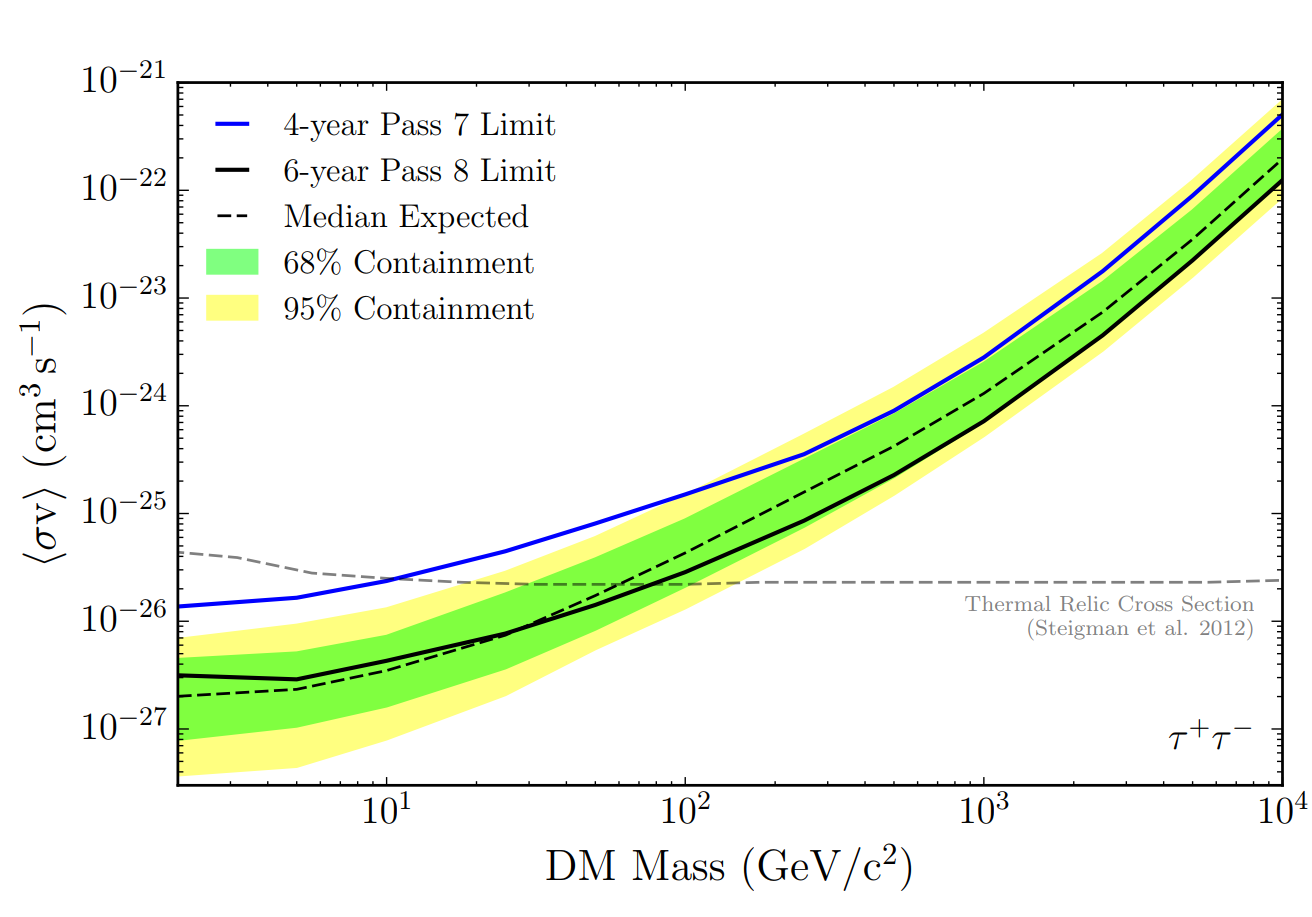
\includegraphics[width=0.54\textwidth]{figures/theory/fermilat.png}
    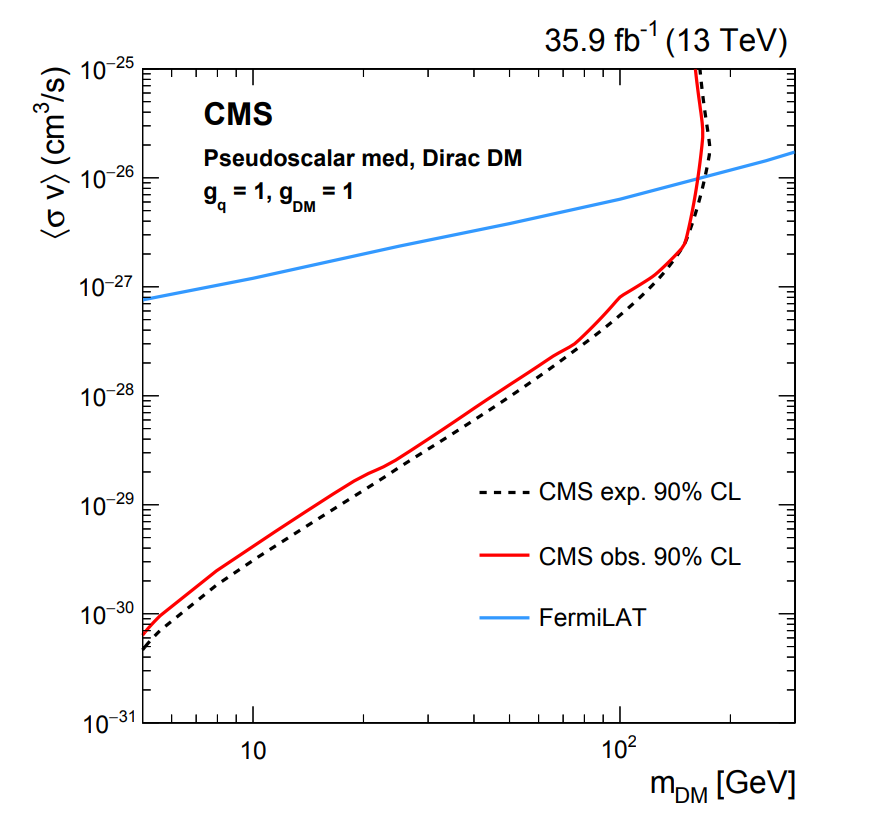
\includegraphics[width=0.4\textwidth]{figures/theory/monojet.png}
    \caption{Excluded WIMP hypotheses as a function of $m_\chi,\langle\sigma v\rangle$ from Fermi-LAT (left) and compared to CMS (right).
             Reprinted from Reference~\cite{fermilat} (left) and Reference~\cite{monojet} (right).}
    \label{fig:theory:fermilat}
\end{center}
\end{figure}

\emph{Direct detection} experiments typically contain a large volume of instrumented material that has a large cross section for interaction with WIMPs.
An example is the Large Underground Xenon (LUX) experiment~\cite{lux}, a two phase (liquid and gas) xenon detector.
LUX searches for scintillation photons and additional electrons emitted from DM-nucleus interactions.
Xenon is chosen because heavy nuclei have larger cross sections for \emph{spin independent} DM interactions.
In this context, spin independent refers to any interaction mediated by a scalar or vector current (i.e. there is no coupling to the spin of the DM or nucleon). 
Figure~\ref{fig:theory:lux} compares the exclusions of LUX to other direct detection experiments.
The results are presented as a function of the natural quantities for direct detection: $m_\chi$ and $\sigma(\chi N \rightarrow \chi N)$.
Also shown is the exclusion limit from the CMS invisible Higgs search, which is described in Chapter~\ref{sec:vbf}.

\begin{figure}[]
    \begin{center}
        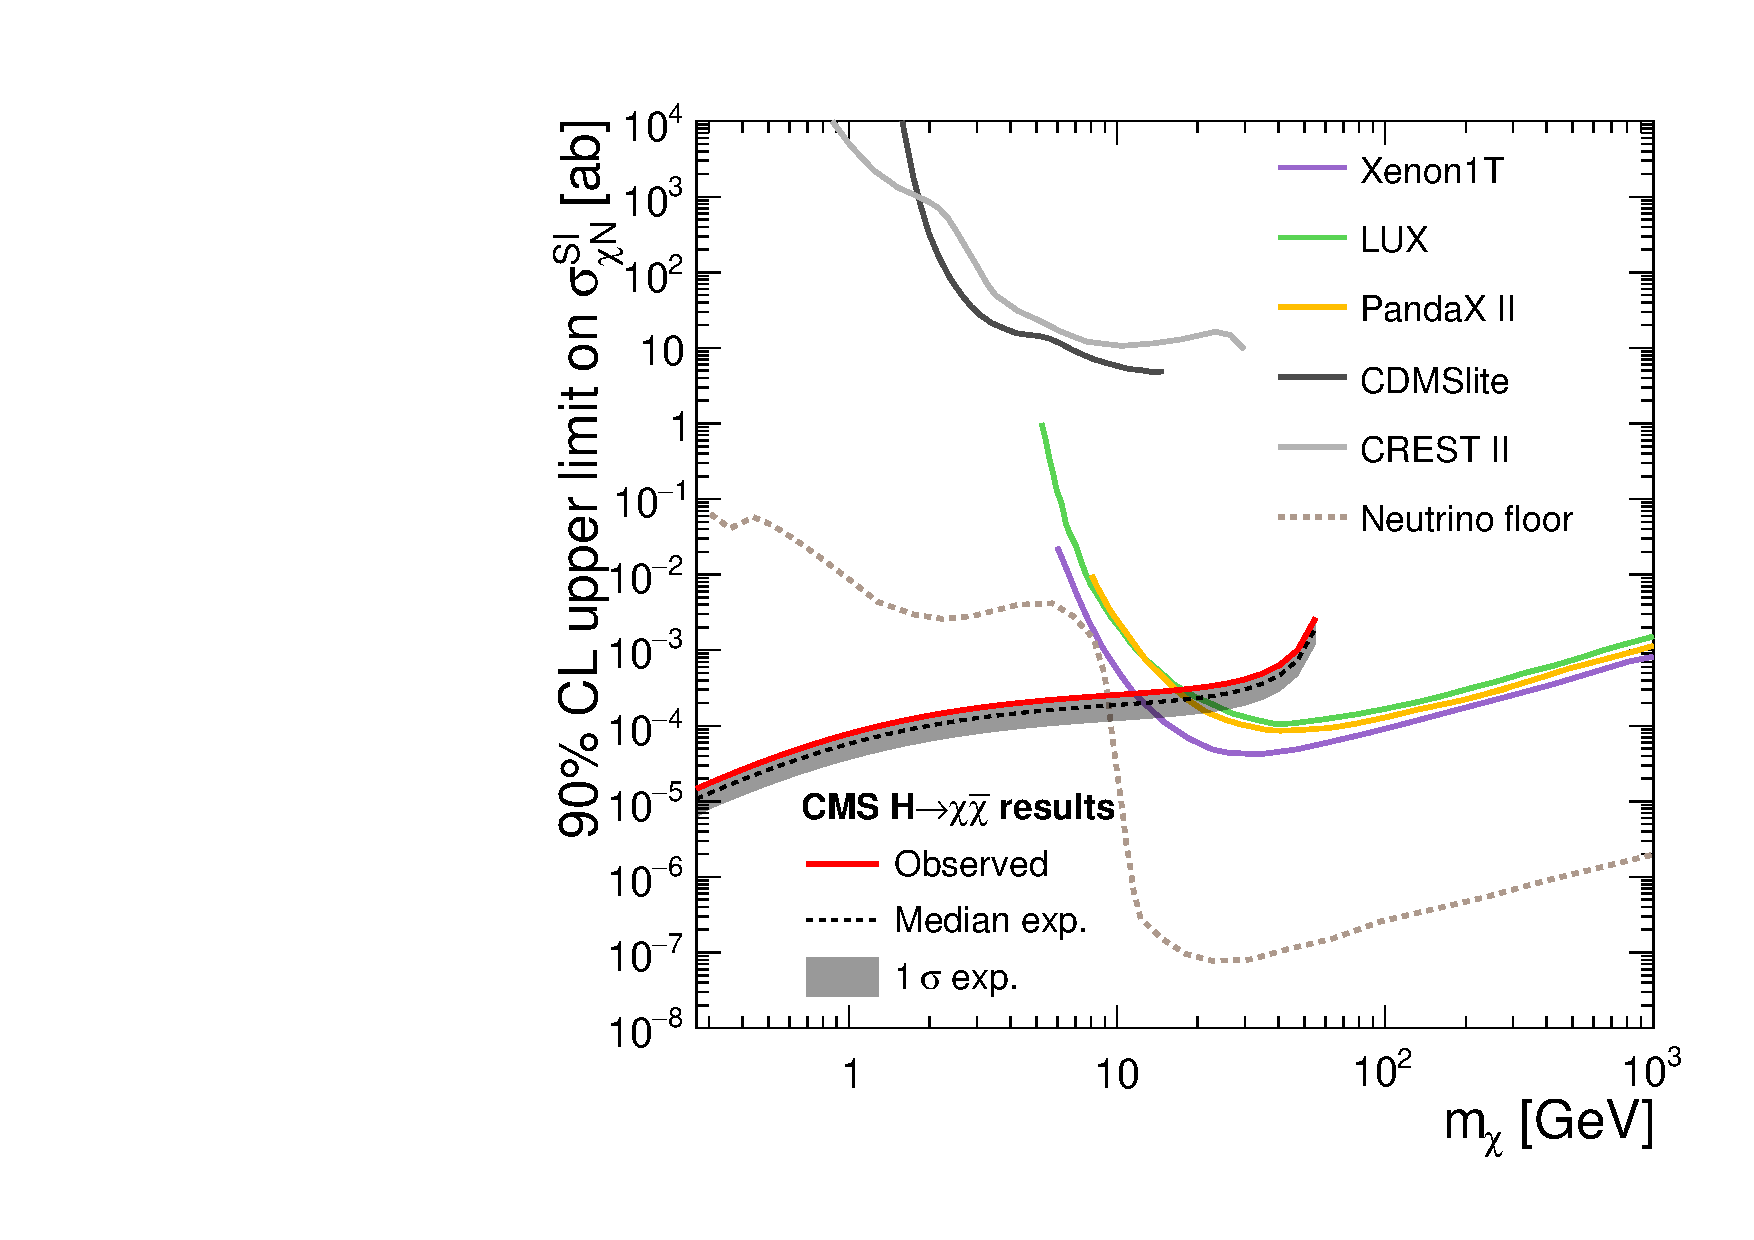
\includegraphics[width=0.5\textwidth]{figures/vbf/fits/dd.pdf}
        \caption{Comparison of various direct detection experiments' sensitivity to WIMP models and the sensitivity of the CMS invisible Higgs search.
                 Details of the CMS curve are presented in Chapter~\ref{sec:vbf}.}
        \label{fig:theory:lux}
    \end{center}
\end{figure}

The results presented in this section suggest that collider searches have complementary sensitivity for certain DM hypotheses, typically at low masses.
The searches described in this thesis target those models, as well as exotic models to which standard direct and indirect detection experiments have very little sensitivity.

\section{LHC phenomenology}

The Large Hadron Collider collides protons at a center of mass energy $\sqrt{s} = 13$ TeV.
Section~\ref{sec:cms:lhc} provides an overview of the LHC machine.
In this section, we describe the methods used to make predictions of observables at the LHC.
These observables typically take the form of differential cross sections $\di\sigma(pp\rightarrow X)/\di\Theta$, where $X$ is some interesting final state with $N$ particles and $\Theta$ is a set of interesting kinematics.
The differential element of the general cross section for $2\rightarrow N$ processes is:
\begin{equation}
\di\sigma(ab\rightarrow \{c_i\}) = 
    \frac{1}{2s} \left(\prod_i \dfrac{\mathrm{d}^3p_i}{(2\pi)^3} \frac{1}{2E_i}\right) 
        \cdot (2\pi)^4 \delta^4\left(k_a + k_b - \sum_i p_i\right) 
        \cdot \left|\Ma(ab\rightarrow \{c_i\})\right|^2
        \label{eq:theory:2n}
\end{equation}
where $k_a,k_b$ are the incoming momenta; $\{p_i\}$ are the outgoing momenta; and $\Ma$ is the matrix element of this reaction.

Hadron collisions do not have two-particle initial states, but rather two composite particles containing partons with varying momenta. 
The general cross section for $pp\rightarrow X$ is~\cite{tasi009}:
\begin{equation}
\di\sigma(pp\rightarrow X(\Theta)) = 
    \sum_{a,b} \int \mathrm{d}x_a \mathrm{d}x_b 
    ~f_a(x_a,\mu_F) f_b(x_b,\mu_F) 
    \cdot \di\sigma(ab\rightarrow\{c_i\}) 
    \cdot D(\{c_i\}\rightarrow X(\Theta))
    \label{eq:theory:master}
\end{equation}
The sum over $a,b$ refers to summing over partons in the initial state.
The momentum fractions of the partons, $x_{a,b}$, follow parton distribution functions (PDFs) $f_{a,b}$ that depend on the particle species $a$ and $b$. 
We then define an intermediate state $\{c_i\}$ which evolves into the final state $X(\Theta)$.
That is, the process $ab\rightarrow X$ is split into $ab\rightarrow \{c_i\} \rightarrow X$.
The definition of $\{c_i\}$ is not unique, but is chosen such that the process $ab\rightarrow\{c_i\}$ can be analyzed perturbatively.
The non-perturbative aspects of evolution to the final state (soft or collinear radiation) will be analyzed separately. 
The matrix element for the first step (\emph{hard scattering}) is computed perturbatively and turned into a cross section by means of Equation~\ref{eq:theory:master}.
Other heuristic methods are used to deal with the second step (\emph{parton shower} (PS)), encoded in the \emph{fragmentation function} $D$. 

The ability to partition the calculation into perturbative (hard scattering) and non-perturbative (PDF and PS) components follows from the collinear factorization theorem~\cite{fact}.
The factorization depends on an arbitrary energy scale $\mu_F$, which defines a lower bound for interactions considered part of the hard scattering. 
The remainder of this section discusses the use of Monte Carlo (MC) methods to simulate these three factors: $f$, $\Ma$, and $D$.

\subsection{Parton distribution functions}
The analytic behavior of PDFs as a function of the factorization scale is governed by the DGLAP evolution equation~\cite{dglap1,dglap2,dglap3}:
\begin{gather}
    \mu_F \frac{\di}{\di\mu_F} f_a(x_a,\mu_F) = \frac{\alpha_S}{\pi} \int_x^1 \frac{\di y}{y} f_a(y,\mu_F) P_{qq} \left(\frac{x}{y}\right) \\
    \text{where } P_{qq}(z) = \frac{4}{3}\left[\frac{1+z^2}{1-z}\right]_+ + 2\delta(1-z) \nonumber 
    \label{eq:theory:dglap}
\end{gather}
The computation of $f_a$ for a fixed scale cannot be done analytically.
Instead, data from many experiments are used to fit a parameterization, as is done by the NNPDF collaboration~\cite{nnpdf}.
Results presented in this thesis use the NNPDF3.0 PDF set.

\subsection{Hard scattering}

Monte Carlo generators simulate Equation~\ref{eq:theory:2n} by sampling events with probability proportional to the phase space and matrix element.
The dedicated MC generators used in this result are MadGraph5~\cite{mg5,fxfx} and Powheg2~\cite{powheg}.
Both generators can simulate to leading order (LO) in EW vertices and up to next-to-leading order (NLO) in QCD vertices.
Finally, the PS model Pythia8.2~\cite{pythia} (discussed in the next section) can also generate certain hard scattering processes at LO in QCD.

MC generators also generate additional partons from initial and final state radiation as part of the hard scattering.
These quarks, gluons, and photons can be highly energetic in events with large $q^2$, and so it is necessary to compute them as part of the hard scattering matrix element.  
It should be noted that, while NLO event generation is always preferable, it comes with two costs: (a) being able to generate fewer additional partons and (b) additional computational time.
We will use LO simulation for processes which have large cross sections and in which additional parton spectra are important.
Table~\ref{tab:theory:sim} provides a summary of the MC generators and orders used in these results.

\begin{table}[]
\begin{center}
    \caption{Summary of MC generators used for each SM and signal process.
             Note that the $V$+jet processes have two entries each in this table, at different QCD orders.
             Both will be used to improve the prediction accuracy.}
    \label{tab:theory:sim}
    \begin{tabular}{c|c|c|l}
        $pp\rightarrow X$ & Generator & NLO in QCD? & Notes \\ \hline \hline
        $t\bar{t}$ & Powheg & \cmark \\ 
        $t$, $tW$, $tZ$ & Powheg & \cmark \\ 
        \hline
        $ZZ,~WZ,~WW$ & Pythia &  \\ 
        \hline
        $Z$ (+0,1 partons) & MG  & \cmark  \\ 
        $W$ (+0,1 partons) & MG  & \cmark \\ 
        $\gamma$ (+0,1 partons) & MG  & \cmark  \\ 
        \hline
        $Z$ (+0,1,2,3 partons) & MG  &  \\ 
        $W$ (+0,1,2,3 partons) & MG  &  \\ 
        $\gamma$ (+0,1,2 partons) & MG  &  \\ 
        Multijet & MG && Jets defined in Section~\ref{sec:theory:ps} \\
        \hline
        Resonant DM & MG && See Chapter~\ref{sec:mt} \\ 
        FCNC DM & MG &\cmark& See Chapter~\ref{sec:mt} \\ 
        VBF $\hinv$ & Powheg && See Chapter~\ref{sec:vbf} \\ 
    \end{tabular}
\end{center}
\end{table}

\subsection{Parton shower}
\label{sec:theory:ps}
Suppose we know $\di\sigma(ab\rightarrow \{c_i\})$ and would like to know $\di\sigma(ab\rightarrow\{c_i\}j)$, where $j$ is radiated from one of the $c_i$ in the soft and/or collinear limit.
Such ``splittings'' include:
\begin{gather}
    q\rightarrow qg, \quad g\rightarrow qq, \quad g\rightarrow gg, \nonumber \\ 
        f\rightarrow f\gamma, \quad \gamma\rightarrow ff 
\end{gather}
Define $z$ to be the fraction of energy kept by the parent parton and $\theta$ to be the opening angle between $c_i$ and $j$. 
For QCD splittings, the cross section can be written (at LO):
\begin{equation}
    \di\sigma(ab\rightarrow\{c_i\}j) =
        P_{c_i \rightarrow c_i j} (z) 
        \cdot \frac{\alpha_S}{2\pi} 
        \cdot \frac{\di\theta}{\theta} 
        ~\di z
        ~\di\sigma(ab\rightarrow\{c_i\})
\end{equation}
where $P_{c_i\rightarrow c_i j}$ are \emph{splitting functions} analogous to the ones that arise in the DGLAP evolution (Equation~\ref{eq:theory:dglap}).
As an example, the splitting function for $q\rightarrow qg$ is~\cite{pythia}:
\begin{equation}
    P_{q\rightarrow qg} = \frac{4}{3} \frac{1+z^2}{1-z}
\end{equation}

It should be noted that this cross section grows as $\theta\rightarrow 0$ and $z\rightarrow 1$, i.e. soft and collinear splittings.
That is, if a bare quark is produced in an event, it will produce many soft and collinear gluons (which in turn can split to $qq$ and $gg$) prior to hadronization.
This iterative process is known as the $\emph{parton shower}$.
As the width of the parton shower nears $1/\Lambda_\mathrm{QCD}$, the partons will hadronize, preventing further splitting.
These hadronic endpoints of the shower reach the detector and appear as collimated sprays of hadrons (\emph{jets}).
The reconstruction of jets is described in detail in Section~\ref{sec:cms:jets} and Chapter~\ref{sec:jets}. 

PS models simulate the shower and hadronization processes.
The results in this thesis use Pythia8.2~\cite{pythia} which employs the Lund string model~\cite{lund} to simulate hadronization.
